\documentclass{standalone}
\usepackage{circuitikz,siunitx}
\usetikzlibrary{shadings,decorations.pathmorphing,arrows.meta,patterns}

\begin{document}
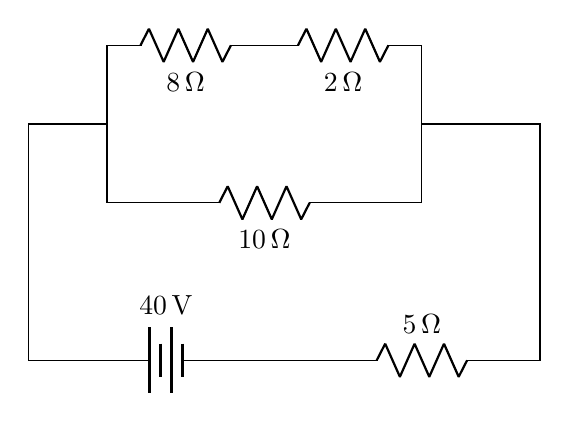
\begin{tikzpicture}
    \draw (0,0)
      to[battery,l=\SI{40}{\volt}] 
                                  ++(3.5,0)
      to[R,l=\SI{ 5}{\ohm}]       ++(3,0)
      to                          ++(0,3)
      to                          ++(-1.5,0)
                                   coordinate (a)
      to                          ++(0,1)
      to[R,l=\SI{ 2}{\ohm}]       ++(-2,0)
      to[R,l=\SI{ 8}{\ohm}]       ++(-2,0)
      to                          ++(0,-1) coordinate (b)
      to                          ++(-1,0)
      to                          ++(0,-3);
    \draw (a) to                  ++(0,-1)
      to[R,l=\SI{10}{\ohm}]       ++(-4,0) to (b);
\end{tikzpicture}
\end{document}